\begin{figure}[t]
  \centering
  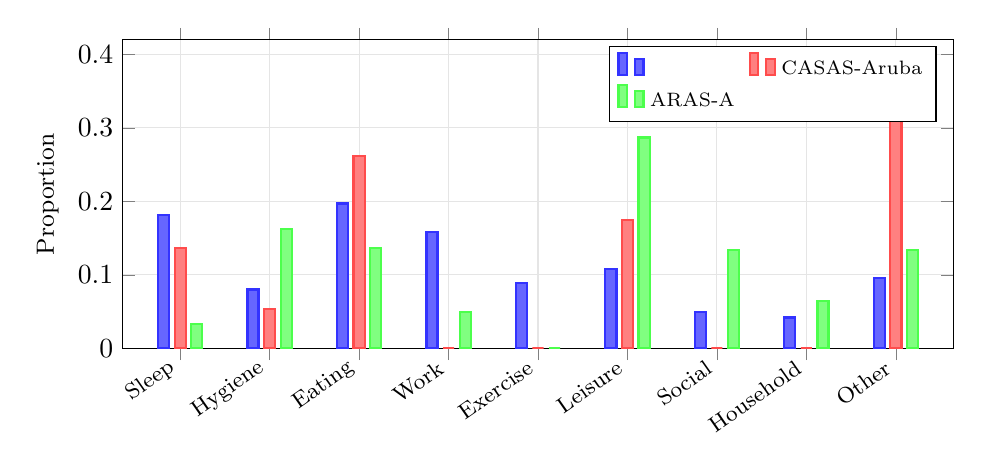
\begin{tikzpicture}
    \begin{axis}[
      ybar,
      width=\columnwidth,
      height=5.5cm,
      bar width=4pt,
      ylabel={Proportion},
      ylabel style={font=\small},
      symbolic x coords={Sleep, Hygiene, Eating, Work, Exercise,
                         Leisure, Social, Household, Other},
      xtick=data,
      x tick label style={rotate=35, anchor=east, font=\footnotesize},
      ytick style={font=\small},
      ymin=0, ymax=0.42,
      legend style={at={(0.98,0.98)}, anchor=north east,
                    font=\scriptsize, legend columns=2,
                    /tikz/every even column/.append style={column sep=3pt}},
      legend cell align=left,
      enlarge x limits=0.08,
      grid=major,
      grid style={gray!20},
      every axis plot/.append style={thick},
    ]
    % VESPER-generated (from rq1 data: 1748 total events)
    \addplot[fill=blue!60, draw=blue!80] coordinates {
      (Sleep,0.181) (Hygiene,0.080) (Eating,0.197)
      (Work,0.158) (Exercise,0.089) (Leisure,0.108)
      (Social,0.049) (Household,0.042) (Other,0.096)
    };
    % CASAS-Aruba (5 categories; missing mapped to 0)
    \addplot[fill=red!50, draw=red!70] coordinates {
      (Sleep,0.137) (Hygiene,0.053) (Eating,0.262)
      (Work,0.000) (Exercise,0.000) (Leisure,0.175)
      (Social,0.000) (Household,0.000) (Other,0.372)
    };
    % ARAS-House A (8 categories)
    \addplot[fill=green!50, draw=green!70] coordinates {
      (Sleep,0.033) (Hygiene,0.162) (Eating,0.137)
      (Work,0.049) (Exercise,0.000) (Leisure,0.287)
      (Social,0.134) (Household,0.064) (Other,0.134)
    };
    \legend{\sys{}, CASAS-Aruba, ARAS-A}
    \end{axis}
  \end{tikzpicture}
  \caption{Activity category distributions for \sys{}-generated schedules
  vs.\ CASAS-Aruba and ARAS-House~A\@.  \sys{} covers all nine categories
  while reference datasets use subsets (5 and 8 categories respectively),
  contributing to the distributional divergence in
  \Cref{tab:activity-realism}.  Zero-valued bars indicate categories absent
  from the reference annotation scheme.}
  \label{fig:activity-dist}
\end{figure}
